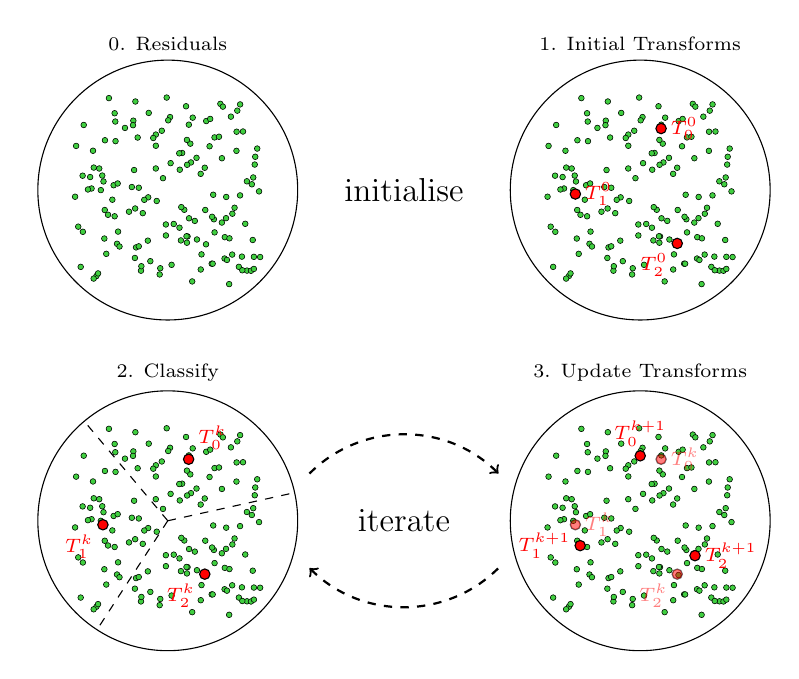
\begin{tikzpicture}[scale=0.6]
	\pgfplotsset{/tikz/font={\scriptsize}}

	% add this node to prevent pdfcrop from cropping the circles
	\draw[black!0] (-2.77,0) node {};

	\pgfmathsetseed{5}
	\foreach \i in {1,2,...,150}{
		\pgfmathsetmacro{\x}{(rand*0.5 + 1)*4 - 4.0}
		\pgfmathsetmacro{\y}{(rand*0.5 + 1)*4 - 4.0}
		\pgfmathsetmacro{\opacVal}{rand*0+1}
		\filldraw [black!25!green!75, opacity = \opacVal] (\x,\y) circle (0.05);
		\draw[very thin] (\x,\y) circle (0.06);
	}

	\draw (0,0) circle [radius=2.75];

	\draw (90:2.75) node [above] {0. Residuals};
	\pgfmathsetseed{5}
	\foreach \i in {1,2,...,150}{
		\pgfmathsetmacro{\x}{(rand*0.5 + 1)*4 - 4.0}
		\pgfmathsetmacro{\y}{(rand*0.5 + 1)*4 - 4.0}
		\pgfmathsetmacro{\opacVal}{rand*0+1}
		\filldraw [black!25!green!75, opacity = \opacVal] (\x+10,\y) circle (0.05);
		\draw[very thin] (\x+10,\y) circle (0.06);
	}

	\draw (10,0) circle [radius=2.75];

	\filldraw [red] (10,0)++(71.25:1.375) circle (0.1) node [right] (T0) {$T_0^0$};
	\draw[thin] (10,0)++(71.25:1.375) circle (0.11);

	\filldraw [red] (10,0)++(183.5:1.375) circle (0.1) node [right] (T1) {$T_1^0$};
	\draw[thin] (10,0)++(183.5:1.375) circle (0.11);

	\filldraw [red] (10,0)++(304.75:1.375) circle (0.1) node [below left] (T2) {$T_2^0$};
	\draw[thin] (10,0)++(304.75:1.375) circle (0.11);

	\draw (10,0)++(90:2.75) node [above] {1. Initial Transforms};

	\draw (5,0) node {\large initialise};

	%%%%%%%%%
	\def\yoffset{-7}

	\pgfmathsetseed{5}
	\foreach \i in {1,2,...,150}{
		\pgfmathsetmacro{\x}{(rand*0.5 + 1)*4 - 4.0}
		\pgfmathsetmacro{\y}{(rand*0.5 + 1)*4 - 4.0 + \yoffset}
		\pgfmathsetmacro{\opacVal}{rand*0+1}
		\filldraw [black!25!green!75, opacity = \opacVal] (\x,\y) circle (0.05);
		\draw[very thin] (\x,\y) circle (0.06);
	}

	\draw (0,\yoffset) circle [radius=2.75];
	\draw[dashed] (0,\yoffset) --++ (12.5:2.75);
	\draw[dashed] (0,\yoffset) --++ (130:2.75);
	\draw[dashed] (0,\yoffset) --++ (237:2.75);

	\filldraw [red] (0,\yoffset)++(71.25:1.375) circle (0.1) node [above right] (T0) {$T_0^k$};
	\draw[thin] (0,\yoffset)++(71.25:1.375) circle (0.11);

	\filldraw [red] (0,\yoffset)++(183.5:1.375) circle (0.1) node [below left] (T1) {$T_1^k$};
	\draw[thin] (0,\yoffset)++(183.5:1.375) circle (0.11);

	\filldraw [red] (0,\yoffset)++(304.75:1.375) circle (0.1) node [below left] (T2) {$T_2^k$};
	\draw[thin] (0,\yoffset)++(304.75:1.375) circle (0.11);

	\draw (0,\yoffset)++(90:2.75) node [above] {2. Classify};
	\pgfmathsetseed{5}
	\foreach \i in {1,2,...,150}{
		\pgfmathsetmacro{\x}{(rand*0.5 + 1)*4 - 4.0}
		\pgfmathsetmacro{\y}{(rand*0.5 + 1)*4 - 4.0 + \yoffset}
		\pgfmathsetmacro{\opacVal}{rand*0+1}
		\filldraw [black!25!green!75, opacity = \opacVal] (\x+10,\y) circle (0.05);
		\draw[very thin] (\x+10,\y) circle (0.06);
	}

	\draw (10,\yoffset) circle [radius=2.75];

	\filldraw [red, opacity=0.5] (10,\yoffset)++(71.25:1.375) circle (0.1) node [right] (T0) {$T_0^k$};
	\draw [thin, opacity=0.5] (10,\yoffset)++(71.25:1.375) circle (0.11);

	\filldraw [red, opacity=0.5] (10,\yoffset)++(183.5:1.375) circle (0.1) node [right] (T1) {$T_1^k$};
	\draw [thin, opacity=0.5] (10,\yoffset)++(183.5:1.375) circle (0.11);

	\filldraw [red, opacity=0.5] (10,\yoffset)++(304.75:1.375) circle (0.1) node [below left] (T2) {$T_2^k$};
	\draw [thin, opacity=0.5] (10,\yoffset)++(304.75:1.375) circle (0.11);

	\filldraw [red] (10,\yoffset)++(90:1.375) circle (0.1) node [above] (T0') {$T_0^{k+1}$};
	\draw [thin] (10,\yoffset)++(90:1.375) circle (0.11);

	\filldraw [red] (10,\yoffset)++(202.5:1.375) circle (0.1) node [left] (T1') {$T_1^{k+1}$};
	\draw [thin] (10,\yoffset)++(202.5:1.375) circle (0.11);

	\filldraw [red] (10,\yoffset)++(327.5:1.375) circle (0.1) node [right] (T2') {$T_2^{k+1}$};
	\draw [thin] (10,\yoffset)++(327.5:1.375) circle (0.11);

	\draw (10,\yoffset)++(90:2.75) node [above] {3. Update Transforms};

	\draw[thick,dashed, ->] (3,\yoffset+1) to[in=135,out=45] ++ (4,0);
	\draw (5,\yoffset) node {\large iterate};
	\draw[thick,dashed, <-] (3,\yoffset-1) to[in=-135,out=-45] ++ (4,0);
\end{tikzpicture}

% vim:set filetype=tex:
